\chapter{Beispiele}

In diesem Abschnitt werden Beispiele zur Nutzung dieser Template dargestellt.
Dieses dient zu einem als Demonstration als auch als rudimentäre Referenz für diese Beispiele.
Damit diese Sektion einen realistischen Anblick erhält, werden die Beispiele mit einer gewissen Menge an bedeutungslosem Blindtext gefüllt.

\section{Inhalte}

\subsection{Symbole}

Diese Template enthält eigene Symbole für verschiedene Dinge, wie zum Beispiel die Programmiersprache \cpp.
Ein anderes Symbol ist der Asterismus, gekennzeichnet durch drei zentrierte Sterne.
Dieser kann als typografischer Dinkus verwendet werden um nach einem Paragrafen zu symbolisieren, dass ein neuer unzusammenhängender Abschnitt beginnt.

\threeast

\enquote{S Nibelungenliad is as bekanntaste boarische und deitsche Hejdnepos (\enquote{Liad} hod im Oidboarischn aa de Bedeitung \enquote{Saga}). Gschriebm worn is am Ofang vom 13. Joarhundat in Boarisch-Middlhochdeitsch.
Es is de Gschicht vom Untagang vom Voik vo de Burgunda, vo da Eamoadung vom Hejdn Siegfried und vo da bluadign Rache vo seim Weib Kriemhild.}
So der Wikipedia Eintrag für das Niebelungenlied auf bayrisch.
Ein Beispiel für den fehlenden Zusammenhang der Paragrafen innerhalb eines Abschnittes markiert durch den Dinkus.

\subsection{Listen}

Für weitere Informationen zur \enquote{korrekten} Nutzung von \LaTeX\ werden folgende Ressourcen vorgeschlagen:

\begin{itemize}
    \item \url{https://github.com/schtandard/latex_primer}
    \item \url{https://tex.stackexchange.com}
    \item Das ist ein längerer Paragraph.
    Dieser Zeigt an, wie das \texttt{itemize} Environemnt mit Paragraphen umgeht.
\end{itemize}

\marginline{Das hier ist eine Randnotiz.}
In dieser Zeile wird eine Randnotiz verwendet.
Diese befinden sich immer am äußeren Seitenrand, damit diese nicht in der Bindung verschwinden.
\footnote{Die Bindungskorrektur dieses Dokuments ist in \texttt{./src/preamble/preamble.tex} mit der \texttt{BCOR} variable standardmäßig auf $15\si{mm}$ gesetzt.}
Es kann natürlich auftreten, dass man auch Fußnoten benutzten möchte, daher das vorherige Beispiel.

\subsection{Akronyme}

Das ist ein \gls{acr}.
Diese kann man in dem \gls{glossary} finden.
Zum ersten Aufruf eines \gls{acr}, wird dieses ausgeschrieben.
Weitere Aufrufe zeigen nur die Kurzfassung (\glsxtrshort{acr}) an.
Jedes Akronym ist auch ein Hyperlink und führt, solange der PDF-Reader dies unterstützt, zurück zur Definition.

\subsection{Abbildungen}

In \autoref{fig:exampleImage} wird ein Beispielbild gezeigt.
Dieses wird aus dem \texttt{/img/} Ordner verwendet.
Das Bild wird automatisch durch \LaTeX\ skaliert.

Die Referenz für das Bild (\autoref{fig:exampleImage} oder nur \ref{fig:exampleImage}) wird im Quellcode mit dem \texttt{\textbackslash autoref\{\}} Kommando gemacht.
Das Argument bezieht sich auf das \texttt{\textbackslash label\{\}} der Abbildung.
Jede \texttt{figure}, \texttt{table}, \texttt{equation}, \texttt{section} und weitere können mit einem Label versehen werden.
Damit kann auf alles referenziert werden.
Das tatsächliche Label, welches vergeben wird, kann frei gewählt werden.
\autoref{fig:exampleImage} wurde hier das Label \enquote{\texttt{fig:exampleImage}} gegeben.
Das Präfix (\texttt{fig:}) hat keine syntaktische Bedeutung für \LaTeX.
Es lohnt sich dennoch verschiedenen Elementen diese Präfixe zu verleihen, um den Überblick nicht zu verlieren.
In \autoref{tab:prefix-table} unter \autoref{sec:tables} werden verschiedene empfohlene Präfixe aufgeführt.

\begin{figure}[ht]
    \centering
    \includegraphics[width=0.8\textwidth]{test.jpg}
    \caption[Beispielbild]{Beispielbild von \citeauthor{exampleImage} aus \autocite{exampleImage}.}
    \label{fig:exampleImage}
\end{figure}

In \autoref{fig:exampleFigure} wird eine Beispielgraph dargestellt.

\begin{figure}[ht]
    \centering
    \begin{subfigure}{0.45\textwidth}
        \begin{tikzpicture}
            \begin{axis}[width=1.0\textwidth]
            \addplot[color=THDGreen]{exp(x)};
            \end{axis}
        \end{tikzpicture}
        \caption{Expontentialfunktion in 2D}
        \label{fig:2d-exp}
    \end{subfigure}
    \begin{subfigure}{0.45\textwidth}
        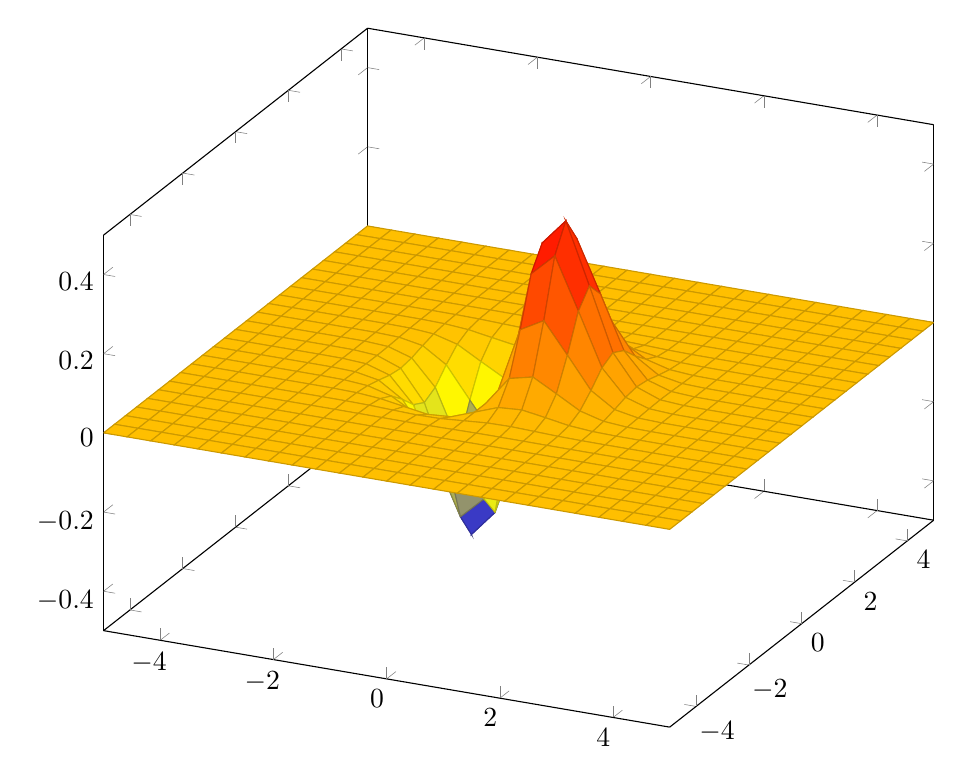
\begin{tikzpicture}
            \begin{axis}[width=1.0\textwidth]
                \addplot3[surf]{exp(-x^2-y^2)*x};
            \end{axis}
        \end{tikzpicture}
        \caption{Expontentialfunktion in 3D}
        \label{fig:3d-exp}
    \end{subfigure}
    \caption[Beispielgraph]{Beispielgraph in \textsc{pgfplots}.}
    \label{fig:exampleFigure}
\end{figure}

\subsubsection{Tikz}

In \autoref{fig:tikz} wird eine CircuitTi\textit{k}Z Zeichnung dargestellt.

\begin{figure}[ht]
    \centering
    \begin{circuitikz}[]
        \draw (0,0)  to[short, o-] (2,0) to[R,l_=$R_1$] (2,-2) to[short,*-o] (3,-2);
        \draw (2,-2) to[R,l_=$R_2$, -*] (2,-4);
        \draw (0,-4) to[short, o-o] (3,-4);
        \draw (0,0)  to[open, l=$U_{\text{in}}$] (0,-4);
        \draw (3,-2) to[open, l=$U_{\text{out}}$] (3,-4);
    \end{circuitikz}
    \caption{Beispielschaltung}
    \label{fig:tikz}
\end{figure}

\subsubsection{Wrapfig}

\lipsum[10]

\begin{wrapfigure}{R}{6cm}
\centering
\vspace{-0.5cm}
\begin{tikzpicture}[node distance=1.3cm,>=stealth',bend angle=45,auto]

    \tikzstyle{place}=[circle,thick,draw=blue!75,fill=blue!20,minimum size=6mm]
    \tikzstyle{red place}=[place,draw=red!75,fill=red!20]
    \tikzstyle{transition}=[rectangle,thick,draw=black!75,
                fill=black!20,minimum size=4mm]

    \tikzstyle{every label}=[red]

    \node [place,tokens=1] (w1)                           {};
    \node [place] (c1) [below of=w1]                      {};
    \node [place] (s)  [below of=c1,label=above:$s\le 3$] {};
    \node [place] (c2) [below of=s]                       {};
    \node [place,tokens=1] (w2) [below of=c2]             {};

    \node [transition] (e1) [left of=c1] {}
    edge [pre,bend left]                  (w1)
    edge [post,bend right]                (s)
    edge [post]                           (c1);

    \node [transition] (e2) [left of=c2] {}
    edge [pre,bend right]                 (w2)
    edge [post,bend left]                 (s)
    edge [post]                           (c2);

    \node [transition] (l1) [right of=c1] {}
    edge [pre]                            (c1)
    edge [pre,bend left]                  (s)
    edge [post,bend right] node[swap] {2} (w1);

    \node [transition] (l2) [right of=c2] {}
    edge [pre]                            (c2)
    edge [pre,bend right]                 (s)
    edge [post,bend left]  node {2}       (w2);
\end{tikzpicture}
\caption{Wrapfigure eines Petrinetzes}
\label{fig:petri}
\end{wrapfigure}

\lipsum[11]
\marginline{Hier ist ein Beispieltext aufgeführt, welche \autoref{fig:petri} umschließt.}
\lipsum[12]

\subsection{Tabelle}
\label{sec:tables}

Es folgt nun eine Tabelle in \autoref{tab:prefix-table}.

\begin{table}[ht]
    \centering
    \begin{tabular}{|l|c|}
        \hline
        \textbf{Typ} & \textbf{Präfix} \\
        \hline \hline
        \texttt{figure} & \texttt{fig:} \\
        \texttt{table} & \texttt{tab:} \\
        \texttt{equation} & \texttt{eq:} \\
        \texttt{section} & \texttt{sec:} \\
        \texttt{lstlisting} & \texttt{code:} \\
        \hline
    \end{tabular}
    \caption{Beispieltabelle für empfohlene Label Präfixe}
    \label{tab:prefix-table}
\end{table}

\subsection{Mathe}

Die Riemannsche Zeta-Funktion ist in \autoref{eq:exampleEquation} aufgeführt.

\setequationentry{Riemannsche Zeta-Funktion.}
\begin{equation}
    \begin{gathered}
        \zeta(s) = \sum_{n=1}^{\infty} \frac{1}{n^s} = \frac{1}{1^s} + \frac{1}{2^s} + \frac{1}{3^s} + \ldots \\[2ex]
        \text{für } \Re(s) > 1 \text{ und dessen analytischer Kontinuation}
    \end{gathered}
    \label{eq:exampleEquation}
\end{equation}

Eine einfachere Formel wird in \autoref{eq:sqrt} gezeigt.

\setequationentry[Text in der Caption des Satz des Pythagoras.]{Gleichungsverzeichniseintrag des Satz des Pythagoras}
\begin{equation}
    c = \sqrt{a^{2} + b^{2}}
    \label{eq:sqrt}
\end{equation}

\subsection{Quellcode}


In \autoref{code:exampleCode} ist Quellcode gezeigt und \autoref{code:latex} wird Quellcode direkt aus einer Datei angezeigt.

\begin{lstlisting}[
    language=C,
    caption={Ein einfacher C code}, language=C++, label=code:exampleCode, float=h
]
#include <stdlib.h>
#include <stdio.h>

int main(void)  {
    printf("Hello World!\n");
    return EXIT_SUCCESS;
}

double example (double(*f)(double)) {
    return (*f)(wert);
}
\end{lstlisting}

\lstinputlisting[
    linerange={228-235}, % actual line numbers in this file
    firstnumber=228,
    caption={\texttt{./reference.tex} Beispiel zum Einbetten von Quellcode aus einer Datei},
    language=TeX,
    label=code:latex,
    float=h
]{./src/mainmatter/reference/reference.tex} % path is relative to main document.tex

\subsection{Timing Diagramm}

In \autoref{fig:timingFig} ist ein Timing Diagramm abgebildet.

\begin{figure}[ht]
    \begin{center}
    \begin{tikztimingtable}[%
        timing/dslope=0.2,
        timing/.style={x=1.6ex,y=2ex},
        x=1ex,
        timing/rowdist=4ex,
        timing/c/rising arrows,
        timing/name/.style={font=\sffamily\scriptsize},
    ]
    % Draw tikztimingtable signals
    \busref{CS} & HHL;16{L};LHH\\
    \busref{SCK} & UULL;16{C};UU\\
    \busref{SO} & UUU;2D{D7};2D{D6};2D{D5};2D{D4};2D{D3};2D{D2};2D{D1};2D{D0};UUU\\
    % Add verticals bars to background
    \extracode
    \begin{pgfonlayer}{background}
        \begin{scope}[semitransparent ,semithick]
            \vertlines[darkgray,dotted]{0,3.2 ,...,36.0}%
        \end{scope}
    \end{pgfonlayer}
    \end{tikztimingtable}
    \end{center}
    \caption{Zeitablauf einer Datenübertragung}
    \label{fig:timingFig}
\end{figure}
